\documentclass{standalone}
\usepackage{tikz}
%\usetikzlibrary{intersections,calc}
\begin{document}

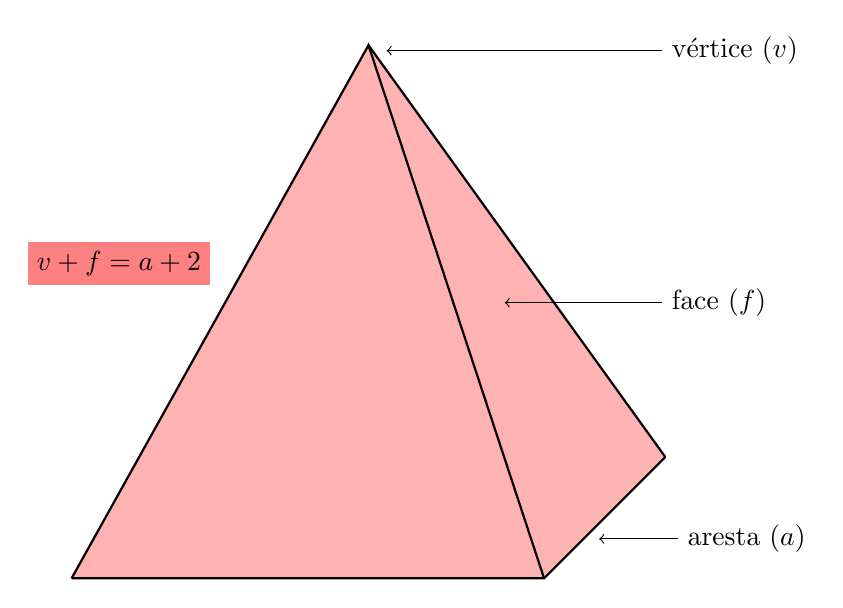
\begin{tikzpicture}
% \draw[help lines,black!30] (-10,-10) grid (10,10);
% \draw[thick,->] (0,-10) -- (0,10) node[left]  {y};
% \draw[thick,->] (-10,0) -- (10,0) node[below] {x};
% \foreach \x in {-10,...,10} \node[left,color=red] at (0,\x) {\x} node[below,color=red] at (\x,0) {\x};
% \node[below right,color=red] at (0,0) {0}; 
           
    % Preenche as faces da pirâmide
   \fill[red!30] (0,3,0) -- (6,3,0) -- (6,3,-4) -- cycle;
   \fill[red!30] (0,3,0) -- (3,9,-2) -- (6,3,0) -- cycle;
   \fill[red!30] (3,9,-2) -- (6,3,0) -- (6,3,-4) -- cycle;
   \draw[<-] (5.5,6.5) -- +(2,0) node[right]       {face ($f$)};
   \draw[<-] (4,9.7)  -- +(3.5,0) node[black,right] {vértice ($v$)};
   \draw[<-] (6.7,3.5) -- +(1,0) node[right]       {aresta ($a$)};
   % Desenha as bordas da pirâmide
   \draw[thick,black] (0,3,0) -- (6,3,0)--(6,3,-4);
   \draw[thick,black] (0,3,0) -- (3,9,-2) -- (6,3,0);
   \draw[thick,black] (3,9,-2) -- (6,3,-4);
   \node[fill=red!50] at (.6,7) {$v + f = a + 2$};
\end{tikzpicture}

\end{document}